\documentclass{article}
\usepackage{amsmath, amssymb}
\usepackage{listings}
\usepackage{color}
\usepackage{graphicx}
\usepackage{geometry}
\usepackage{hyperref}

\geometry{margin=1in}

\definecolor{codegray}{rgb}{0.5,0.5,0.5}
\definecolor{codepurple}{rgb}{0.58,0,0.82}

\lstdefinestyle{mystyle}{
    basicstyle=\ttfamily\footnotesize,
    keywordstyle=\color{blue},
    commentstyle=\color{codegray},
    stringstyle=\color{codepurple},
    breaklines=true,
    frame=single,
    numbers=left,
    numberstyle=\tiny\color{codegray},
    tabsize=2,
}

\lstset{style=mystyle}

\title{Building a Graph Visualization Interface with Tkinter: A Step-by-Step Guide}
\author{}
\date{}

\begin{document}

\maketitle

\tableofcontents

\section{Introduction}

In this guide, we will build a Python application using Tkinter to create a graphical interface for constructing graphs and visualizing graph traversal algorithms like Depth-First Search (DFS), Recursive DFS, and Breadth-First Search (BFS). We will start by setting up the general interface, progressively adding functionality and complexity, and explain each step in detail.

\section{Objectives}

Our main objectives are:

\begin{itemize}
    \item Create a resizable GUI interface with a canvas on the left and controls on the right.
    \item Implement functionality to draw nodes and edges on the canvas.
    \item Allow users to move nodes and update connected edges accordingly.
    \item Integrate graph traversal algorithms and visualize them on the canvas.
\end{itemize}

\begin{figure}[h]
    \centering
    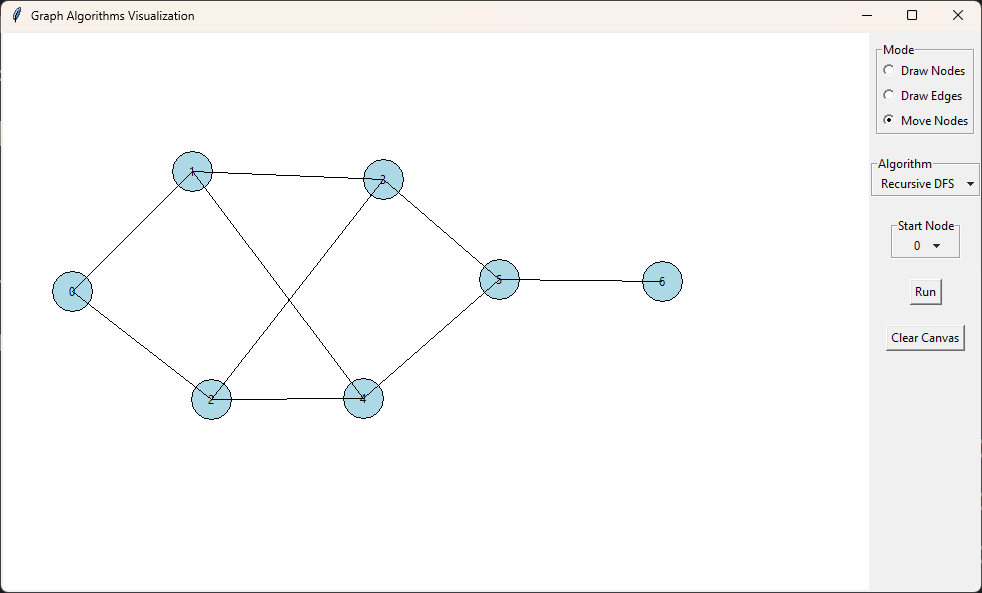
\includegraphics[width=0.8\linewidth]{images/final.png}
    \caption{Final interface}
    \label{fig:final_interface}
\end{figure}
\section{Setting Up the General Interface}

We begin by creating the general structure of the interface, which includes a canvas for drawing and a control panel for user interactions.

\subsection{Importing Necessary Modules}

First, import the necessary modules:

\begin{lstlisting}[language=Python]
import tkinter as tk
from tkinter import ttk
\end{lstlisting}

\subsection{Initializing the Main Application Window}

We create the main application window and set its title.

\begin{lstlisting}[language=Python]
root = tk.Tk()
root.title("Graph Visualization Tool")
root.mainloop()
\end{lstlisting}

\subsection{Creating the Main Frames}

To organize the layout, we use frames. We'll have a main frame that contains two sub-frames: one for the canvas and one for the controls. \\

More information about frames: \href{https://pythonbasics.org/tkinter-frame/}{Tkinter frame}.

\begin{lstlisting}[language=Python]
# Create main frame
main_frame = tk.Frame(root)
main_frame.pack(fill=tk.BOTH, expand=True)
\end{lstlisting}

\subsection{Adding the Canvas and Control Panel}

We add a canvas on the left and a control panel on the right.

\begin{lstlisting}[language=Python]
# Create canvas frame
canvas_frame = tk.Frame(main_frame)
canvas_frame.pack(side=tk.LEFT, fill=tk.BOTH, expand=True)

# Create control frame
control_frame = tk.Frame(main_frame)
control_frame.pack(side=tk.RIGHT, fill=tk.Y)
\end{lstlisting}

In order to visualize the structure we can add some dimensions and colors, in Fig. [\ref{fig:general structure}], we can see the GUI generated so far.

\begin{lstlisting}[language=Python]
import tkinter as tk
from tkinter import ttk

root = tk.Tk()
root.title("Graph Visualisation Tool")

# Create main frame
main_frame = tk.Frame(root)
main_frame.pack(fill=tk.BOTH, expand=True)

# Create canvas frame
canvas_frame = tk.Frame(main_frame, height=100, width=200, bg='red')
canvas_frame.pack(side=tk.LEFT, fill=tk.BOTH, expand=True)

# Create control frame
control_frame = tk.Frame(main_frame, height=100, width=100, bg='blue')
control_frame.pack(side=tk.RIGHT, fill=tk.Y)
root.mainloop()
\end{lstlisting}

\begin{figure}
    \centering
    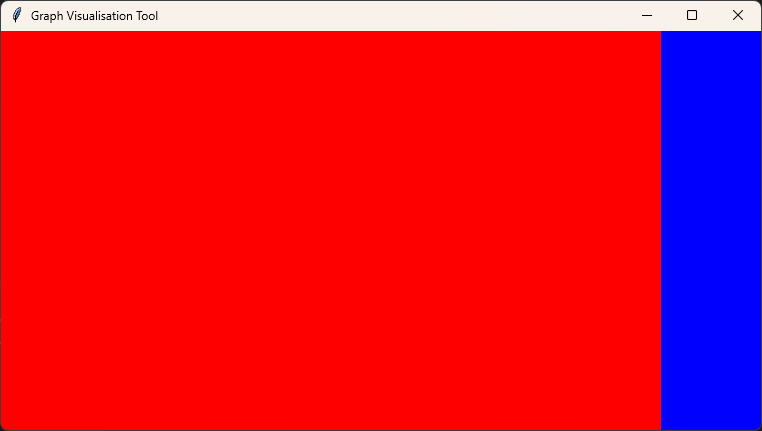
\includegraphics[width=0.5\linewidth]{images/general structure.png}
    \caption{General Structure}
    \label{fig:general structure}
\end{figure}

\subsection{Creating the Canvas}
We create a canvas widget within the canvas frame.

\begin{lstlisting}[language=Python]
canvas = tk.Canvas(canvas_frame, bg="white")
canvas.pack(fill=tk.BOTH, expand=True)
\end{lstlisting}

\subsection{Adding Controls to the Control Panel}
\subsubsection{Mode Radio List}
\begin{figure}[h]
    \centering
    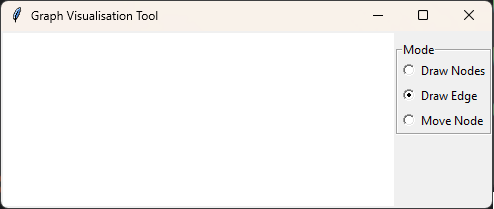
\includegraphics[width=0.5\linewidth]{images/mode_selector.png}
    \caption{Mode Selector}
    \label{fig:mode_selector}
\end{figure}
We can now add buttons, labels, and other widgets to the control panel.

\begin{lstlisting}[language=Python]
# Example control: Mode selection
mode_frame = tk.LabelFrame(control_frame, text="Mode")
mode_frame.pack(pady=10)

node_var = tk.StringVar()
node_var.set("Draw Edge")

draw_node_radio = tk.Radiobutton(mode_frame, text="Draw Nodes", variable=node_var, value="Draw Nodes")
draw_edge_radio = tk.Radiobutton(mode_frame, text="Draw Edge", variable=node_var, value="Draw Edge")
move_node_radio = tk.Radiobutton(mode_frame, text="Move Node", variable=node_var, value="Move Node")

draw_node_radio.pack(anchor=tk.W)
draw_edge_radio.pack(anchor=tk.W)
move_node_radio.pack(anchor=tk.W)
\end{lstlisting}

We can shorten the code by directly packing the Radio Butons on their creation.

\begin{lstlisting}
mode_frame = tk.Label(control_frame, text="Mode")
mode_frame.pack(pady=10)

node_var = tk.StringVar()
node_var.set("Draw Edge")

tk.Radiobutton(mode_frame, text="Draw Nodes", variable=node_var, value="Draw Nodes").pack(anchor=tk.W)
tk.Radiobutton(mode_frame, text="Draw Edge", variable=node_var, value="Draw Edge").pack(anchor=tk.W)
tk.Radiobutton(mode_frame, text="Move Node", variable=node_var, value="Move Node").pack(anchor=tk.W)
\end{lstlisting}

\subsubsection{Algorithm Selection Drop List \& Start Node Drop List}

\begin{figure}[h]
    \centering
    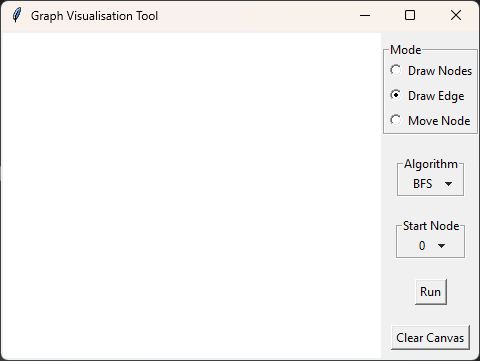
\includegraphics[width=0.5\linewidth]{images/completed_control.png}
    \caption{All Controls}
    \label{fig:all_controls}
\end{figure}

Algorithm selection 
\begin{lstlisting}
algorithms = ["Recursive DFS", "DFS", "BFS"]
selected_alg = tk.StringVar()
alg_menu = ttk.OptionMenu(alg_frame, selected_alg, "BFS", *algorithms)
alg_menu.pack()

start_node_frame = tk.LabelFrame(control_frame, text="Start Node")
start_node_frame.pack(pady=10)
\end{lstlisting}

Node Selection
\begin{lstlisting}
start_node_frame = tk.LabelFrame(control_frame, text="Start Node")
start_node_frame.pack(pady=10)

start_node = tk.IntVar()

start_node_menu = ttk.OptionMenu(start_node_frame, start_node)
start_node_menu.pack()    
\end{lstlisting}
\subsubsection{Run \& Clear Canvas Buttons}
It must be mentioned, that the button also support biding to methods via the parameter command. We will see in the future chapters.

\begin{lstlisting}
# Run button
run_button = tk.Button(control_frame, text="Run")
run_button.pack(pady=10)

# Clear Canvas button
clear_button = tk.Button(control_frame, text="Clear Canvas")
clear_button.pack(pady=10)
\end{lstlisting}

\section{Implementing Canvas Interactions}

Now that we have the basic interface, we can add functionality to interact with the canvas, such as drawing nodes and edges.

\subsection{Rendering a Circle (Node) on the Canvas}

\begin{figure}[h]
    \centering
    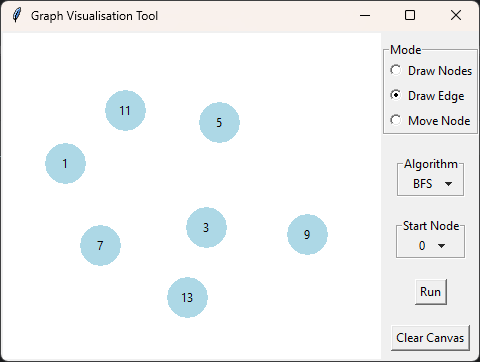
\includegraphics[width=0.5\linewidth]{images/draw_nodes.png}
    \caption{Draw Nodes in Canvas}
    \label{fig:draw_canvas}
\end{figure}
We define a function to draw a node at the position where the user clicks.

\begin{figure}
    \centering
    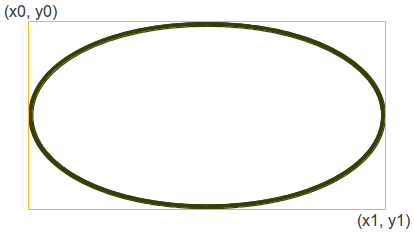
\includegraphics[width=0.5\linewidth]{images/canvas_oval.png}
    \caption{Coordinates on the circle.\\ Source: \href{https://python-course.eu/tkinter/canvas-widgets-in-tkinter.php}{Python-Course Eu Website. Canvas Widgets in Tkinter.}}
    \label{fig:enter-label}
\end{figure}
\begin{lstlisting}[language=Python]
def add_node(event):
    x,y = event.x, event.y
    r = 20
    # id    =        create_oval(x0,    y0,    x1,    y1,    option, ...)
    node_id = canvas.create_oval(x - r, y - r, x + r, y + r, fill="lightblue", outline="lightblue")
    canvas.create_text(x, y, text=str(node_id))
\end{lstlisting}

\subsection{Binding Mouse Events to the Canvas}

We bind the left mouse button click to the \texttt{add\_node} function.

\begin{lstlisting}[language=Python]
canvas.bind("<Button-1>", add_node)
\end{lstlisting}

\subsection{Implementing Node Movement}

We can allow nodes to be moved by clicking and dragging.

\begin{lstlisting}[language=Python]
# Variables to store the selected node
selected_node = None

def select_node(event):
    global selected_node
    # Find the node under the cursor
    items = canvas.find_overlapping(event.x, event.y, event.x, event.y)
    for item in items:
        if canvas.type(item) == "oval":
            selected_node = item
            break

def move_node(event):
    if selected_node:
        x, y = event.x, event.y
        r = 20  # Node radius
        canvas.coords(selected_node, x - r, y - r, x + r, y + r)
        # Update the position of the text label if any

def release_node(event):
    global selected_node
    selected_node = None

# Bind the events
canvas.bind("<Button-1>", select_node)
canvas.bind("<B1-Motion>", move_node)
canvas.bind("<ButtonRelease-1>", release_node)
\end{lstlisting}

\section{Enhancing the Interface}


\end{document}
